\usepackage{xcolor}
\usepackage{layouts}
\usepackage{minted}
\usepackage[most]{tcolorbox}
\usepackage{natbib}
\tcbuselibrary{minted}
\usemintedstyle{xcode}
\setminted{
    fontfamily=helvetica
}

\usepackage{booktabs}

\usepackage{outlines}
\usepackage{hyperref}
\usepackage{graphicx}
\usepackage{amsmath}
\usepackage{makecell}

\renewcommand\theadalign{bc}
\renewcommand\theadfont{\bfseries}
\renewcommand\theadgape{\Gape[4pt]}
\renewcommand\cellgape{\Gape[4pt]}

\beamertemplatenavigationsymbolsempty

\newif\ifsectiontitlepage
\sectiontitlepagetrue

\newcommand{\nosectiontitlepage}{\sectiontitlepagefalse}


\AtBeginSection[]{
\ifsectiontitlepage
  \begin{frame}
  \tableofcontents[currentsection, hideothersubsections]
  \end{frame}
\fi
}



%%

% color
\definecolor{coreFontMain}{RGB}{26,26,26}
\definecolor{coreFontSub}{RGB}{106,106,106}
\definecolor{coreBackgroundLight}{RGB}{230,230,230}
\definecolor{coreBackground}{RGB}{255,255,255}

% heading
\newlength{\headerheight}
\setlength{\headerheight}{0.094\paperheight}


\setbeamerfont{frametitle}{size=\fontsize{12}{14.4}}
\setbeamertemplate{frametitle}
{%
\nointerlineskip
\begin{beamercolorbox}[wd=\paperwidth,left,sep=0pt]{}
\begin{tcolorbox}[enhanced,frame hidden, 
    borderline south={0.5pt}{0pt}{coreFontSub},
    colback=coreBackground, coltext=coreFontSub,height=\headerheight,notitle,left*=0.05\paperwidth,boxsep=0pt,bottom=0pt,halign=left,valign=bottom,before skip=0pt,after skip=0pt, before upper=\strut]
    \usebeamercolor{frametitle}\insertframetitle
\end{tcolorbox}
\end{beamercolorbox}
}


% footer
\newlength{\footerheight}
\setlength{\footerheight}{0.04\paperheight}
\setbeamercolor{footer}{bg=coreBackgroundLight, fg=coreFontMain}

\setbeamertemplate{footline}
{%
\begin{beamercolorbox}[sep=0pt,wd=\paperwidth,center]{footer}
\begin{minipage}[c][\footerheight]{\textwidth}
    \centering
    \insertframenumber/\inserttotalframenumber
\end{minipage}
\end{beamercolorbox}
}



% Title Page

% header
% \newlength{\titleheaderheight}
% \setlength{\titleheaderheight}{0.0666667\paperheight}
% \setbeamercolor{header}{bg=coreBackgroundLight}

%% logo
\newlength{\logoheight}
\setlength{\logoheight}{0.297\paperheight}

%% title
\setbeamercolor{title}{fg=coreFontMain}
\setbeamerfont{title}{size=\fontsize{18.14}{21.768}}
\newlength{\titleheight}
\setlength{\titleheight}{0.19\paperheight}


%% meta
\newlength{\metaheight}
\setlength{\metaheight}{0.21\paperheight}
\setbeamercolor{meta}{fg=coreFontSub}
\setbeamerfont{meta}{size=\fontsize{9.07}{10.884}}

%% contact
\newlength{\contactheight}
\setlength{\contactheight}{0.193333\paperheight}



\makeatletter
% \newcommand{\iftitlegraphicisempty}{%
%   \ifx\@empty\inserttitlegraphic%
%     \expandafter\@firstoftwo%
%   \else%
%     \expandafter\@secondoftwo%
%   \fi%
% }
\setbeamertemplate{title page}{
% \nointerlineskip
% 
\ifx\@empty\inserttitlegraphic%
    \setlength{\titleheight}{0.4\paperheight}
    \setlength{\metaheight}{0.4\paperheight}%
    \setbeamerfont{meta}{size=\fontsize{11}{13.2}}
\else%
    \inserttitlegraphic%
\fi%

\begin{tcolorbox}[enhanced,frame hidden, borderline south={0.5pt}{0pt}{coreFontMain}, colback=coreBackground,height=\titleheight,boxsep=0pt,notitle,halign=flush center,valign=center, bottom=-30pt,before skip=0pt,after skip=0pt, coltext=coreFontMain]
\usebeamercolor{title}
\usebeamerfont{title}\inserttitle
\end{tcolorbox}

\usebeamercolor[fg]{meta}{
\begin{minipage}[c][\metaheight]{\textwidth}
    \usebeamerfont{meta}
    \centering
    \insertauthor \linebreak
    \insertinstitute \linebreak
    \insertdate
\end{minipage}
}


\begin{tcolorbox}[enhanced,frame hidden, colback=coreBackground,height=\contactheight,notitle,halign=flush center,valign=top,before skip=0pt,after skip=0pt,top=-5pt]
\begin{tabular}{ccc}
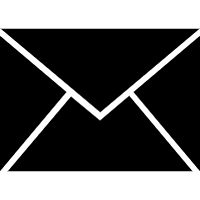
\includegraphics[height=3mm]{bohanbeamerstyle/figures/mail.png} & 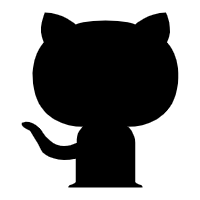
\includegraphics[height=3mm]{bohanbeamerstyle/figures/github.png} &
\includegraphics[height=3mm]{bohanbeamerstyle/figures/Twitter.png}
\end{tabular}

\end{tcolorbox}


% \begin{beamercolorbox}[sep=2pt,center,wd=\paperwidth,ht=\footerheight]{footer}
% \tiny
% \insertframenumber/\inserttotalframenumber
% \end{beamercolorbox}
% \nointerlineskip
}


% 
\setbeamercolor{normal text}{bg=coreBackground,fg=coreFontMain}

% itemize
\setbeamertemplate{itemize items}[circle]

\setlength{\leftmarginii}{10pt}
\setbeamercolor{itemize item}{fg=coreFontMain}
\setbeamercolor{itemize subitem}{fg=coreFontMain}
\setbeamercolor{itemize subsubitem}{fg=coreFontMain}


